\documentclass[11pt,handout,aspectratio=169]{beamer}


%%%%%%%%% GENERAL PACKAGES
%\usepackage{xcolor}
%\usepackage{pdfpages}
%\usetheme[progressbar=frametitle]{metropolis}
%\setbeamercolor{background canvas}{bg=white}
%\usepackage{appendixnumberbeamer}
%\usepackage{booktabs}
%\usepackage[scale=2]{ccicons}
%\usepackage{pgfplots}
%\usepgfplotslibrary{dateplot}
%\usepackage{xspace}
%\newcommand{\themename}{\textbf{\textsc{metropolis}}\xspace}
%\usepackage[absolute,overlay]{textpos}

%%%%%%%%% COLOR THEME

% Define some colors:
\definecolor{DarkFern}{HTML}{407428}
\definecolor{DarkCharcoal}{HTML}{4D4944}
\definecolor{AlertColor}{RGB}{89,124,158}
\definecolor{HighLight}{RGB}{96,95,134}
\definecolor{Important}{RGB}{234,122,133}
\definecolor{Yellow}{HTML}{00539C}
\colorlet{Fern}{DarkFern!85!white}
\colorlet{Charcoal}{DarkCharcoal!85!white}
\colorlet{LightCharcoal}{Charcoal!50!white}
\colorlet{HighLight2}{AlertColor}
\colorlet{DarkRed}{red!70!black}
\colorlet{DarkBlue}{blue!70!black}
\colorlet{DarkGreen}{green!70!black}
\definecolor{RoyalBlue}{HTML}{00539C}
\definecolor{Peach}{HTML}{EEA47F}
\definecolor{ForestGreen}{HTML}{2C5F2D}
\definecolor{MossGreen}{HTML}{E8FCC9}
% Use the colors:
\setbeamercolor{title}{fg=Fern}
\setbeamercolor{frametitle}{fg=MossGreen,bg=ForestGreen}
\setbeamercolor{normal text}{fg=Charcoal!70!black}
\setbeamercolor{block title}{fg=black,bg=Fern!25!white}
\setbeamercolor{block body}{fg=black,bg=Fern!10!white}
\setbeamercolor{block title alerted}{fg=black,bg=DarkRed!25!white}
\setbeamercolor{block body alerted}{fg=black,bg=DarkRed!10!white}
\setbeamercolor{alerted text}{fg=DarkRed}
\setbeamercolor{itemize item}{fg=Charcoal}



%%%%%%%%% OTHER COMMANDS
\newcommand{\indep}{\perp\!\!\! \perp}
\newcommand{\comment}[1]{}
\newcommand{\bs}{\boldsymbol}
\newcommand{\tr}{\text{trace}}
\newcommand{\sgn}{{\rm sgn}}
\def\T{\top}
%\newcommand{\det}{\text{det}}
\newcommand{\var}{\mathrm{var}}
\newcommand{\cC}{{\cal C}}
\newcommand{\cG}{{\cal G}}
\newcommand{\cV}{{\cal V}}
\newcommand{\cE}{{\cal E}}
\newcommand{\cM}{{\cal M}}
\newcommand{\cP}{{\cal P}}
\newcommand{\cX}{{\cal X}}
\newcommand{\cY}{{\cal Y}}
\newcommand{\X}{\mathbf{X}}
\newcommand{\Y}{\mathbf{Y}}
\newcommand{\x}{\mathbf{x}}
\newcommand{\y}{\mathbf{y}}
\newcommand{\z}{\mathbf{z}}

\newcommand{\argmin}{\operatornamewithlimits{argmin}}
\newcommand{\eps}{\varepsilon}
\newcommand{\<}{\langle}
\renewcommand{\>}{\rangle}


\setbeamertemplate{itemize subitem}{\tiny\raise1.5pt\hbox{\donotcoloroutermaths$\blacktriangleright$}}
\setbeamertemplate{itemize subsubitem}{\tiny\raise1.5pt\hbox{\donotcoloroutermaths$\blacktriangleright$}}
\setbeamertemplate{enumerate item}{\insertenumlabel.}
\setbeamertemplate{enumerate subitem}{\insertenumlabel.\insertsubenumlabel}
\setbeamertemplate{enumerate subsubitem}{\insertenumlabel.\insertsubenumlabel.\insertsubsubenumlabel}
\setbeamertemplate{enumerate mini template}{\insertenumlabel}

\newcommand{\TODO}[1]{{\color{red}{[TODO: #1]}}}


\newcommand{\R}{\mathbb R}
\newcommand{\E}{\mathbb E}
\renewcommand{\P}{\mathbb P}


\DeclareMathOperator*{\cov}{cov}


\newsavebox{\zerobox}
\newenvironment{nospace}
{\par\edef\theprevdepth{\the\prevdepth}\nointerlineskip
  \setbox\zerobox=\vtop to 0pt\bgroup
  \hrule height0pt\kern\dimexpr\baselineskip-\topskip\relax
}
{\par\vss\egroup\ht\zerobox=0pt \wd\zerobox=0pt \dp\zerobox=0pt
  \box\zerobox}

\usepackage{soul}
\makeatletter
\let\HL\hl
\renewcommand\hl{%
  \let\set@color\beamerorig@set@color
  \let\reset@color\beamerorig@reset@color
  \HL}
  \makeatother


\title[STA437-Week1]{STA 437/2005: \\ Methods for Multivariate Data}
\subtitle[]{Week 5: Non-Gaussian Distributions}
\author[Piotr Zwiernik]{Piotr Zwiernik}
\institute[UofT]{University of Toronto}
\date{}


%\usepackage{Sweave}

\begin{document}

\maketitle

\begin{frame}{Modelling non-Gaussian distributions}
	Gaussian distribution has many properties that makes it very appealing.\\[2mm]
	
	It does however has some limitations:
	\begin{itemize}
		\item Problem with multimodal populations.
		\item Problem with asymetric distributions.
		\item Not suitable for modelling processes with extreme events. \\[3mm]
	\end{itemize}
	
	\alert{Goal:} Retain some of the advantages of the Gaussian removing some of its limitations.\\[3mm]
	We focus on three approaches: 
	\begin{itemize}
		\item spherical and elliptical distributions
		\item copula modelling
		\item Gaussian mixtures
	\end{itemize}
\end{frame}


\begin{frame}{Table of contents}
\setbeamertemplate{section in toc}[sections numbered]
\tableofcontents%[hideallsubsections]
\end{frame}


\section{Elliptical distributions}

\begin{frame}{}
	\begin{center}
		{\Huge \alert{Elliptical distributions}}
	\end{center}
\end{frame}

\subsection{Spherical distributions}

\begin{frame}{Why Study Elliptical Distributions?}
    \begin{itemize}
        \item Generalize the multivariate normal distribution.\\[5mm]
        \item Model data with heavy tails or outliers.
        \begin{itemize}
        \item higher probability of extreme events\\[5mm]
        \end{itemize}
        \item Maintain symmetry and linear correlation structures.\\[5mm]
        \item Applications in finance, insurance, and environmental studies.
    \end{itemize}
\end{frame}

% Slide: Spherical Distributions Definition
\begin{frame}{Spherical Distributions}
\textbf{Orthogonal Matrices:} $O(m) = \{ U \in \mathbb{R}^{m \times m} : U^\top U = I_m \}$.
%  \begin{itemize}
%    \item $U \in O(m)$ implies $U^{-1} = U^\top$.
%    \item Determinants satisfy $|\det(U)| = 1$.
%  \end{itemize}
\begin{alertblock}{Spherical distribution}
A random vector $X \in \mathbb{R}^m$ has a \emph{spherical distribution} if for any $U \in O(m)$:
  \begin{equation*}
    X \overset{d}{=} U X.
  \end{equation*}	
\end{alertblock}
\textbf{\alert{Example:}} $X\sim N_m(\bs 0,I_m)$ or more generally $X\sim N_m(\bs 0,\sigma^2 I_m)$.
\begin{block}{Density generator and dependence on the norm}
	Characteristic function satisfies: $\psi_X(\bs t)=\psi_{UX}(\bs t)=\psi_X(U^\top \bs t)$ and so \textbf{equivalently} $\psi_X(\bs t)$ depends only on $\|\bs t\|$. The same applies to the density: $$f_X(\x)\;=\;h(\|\bs x\|)\qquad\mbox{for some }h\mbox{ (generator)}.$$
\end{block}
%e.g. $X\sim N_m(\bs 0_m,I_m)$ then $h(s)=\tfrac{1}{(2\pi)^{m/2}}e^{-\tfrac12 s}$
  \end{frame}

% Slide: Examples of Spherical Distributions
\begin{frame}{Examples of Spherical Distributions}
The case $X\sim N_m(\bs 0,\sigma^2 I_m)$ has a simple generalization.\\[3mm]
\begin{block}{Spherical scale mixture of normals}
	If $Z \sim N_m(0, I_m)$ and a random variable $\tau > 0$ is independent of $Z$, then:
      \begin{equation*}
        X = \frac{1}{\sqrt{\tau}} Z
      \end{equation*}
      has a spherical distribution.
\end{block}
  \textbf{Indeed:} Let $U \in O(m)$, then 
$$    UX \;=\; \frac{1}{\sqrt{\tau}} UZ \;\overset{d}{=}\; \frac{1}{\sqrt{\tau}} Z \;=\; X.$$
\end{frame}

% Slide: Moment Structure of Spherical Distributions
\begin{frame}{Moment Structure of Spherical Distributions}
\begin{alertblock}{Spherical symmetry implies:}
  $\bullet$\quad      $\mu\;=\;\mathbb{E}[X] \;=\; 0$, \\
  $\bullet$\quad      $\Sigma\;=\;\var(X) \;=\; c I_m$, \quad for some $c \geq 0$. 
      \end{alertblock}
      \medskip
      
      \textbf{Indeed:} Let $\Sigma=\textcolor{blue}{U\Lambda U^\top} $ be the spectral decomposition.
      \begin{itemize}
      	\item $\Sigma=\var(X)=\var(VX)=V \var(X)V^\top=V\textcolor{blue}{U\Lambda U^\top} V^\top$ for any $V\in O(m)$.
      	\item take $V=U^\top$ to show that $\Sigma$ must be diagonal, $\Sigma=\Lambda$.
      	\item take $V$ to be all the \alert{permutation matrices} to conclude that $\Lambda=c I_m$.  
      \end{itemize} 
%\bigskip
%
%For $X = \frac{1}{\sqrt{\tau}} Z$ with $Z \sim N(0, I_m)$, $\tau>0$, $\tau\indep Z$:
%      \begin{equation*}
%        \var(X) = \mathbb{E}[\tau^{-1}] I_m.
%      \end{equation*}
%\textbf{Indeed:} $\E[X]=\E[\tfrac{1}{\sqrt{\tau}}Z]=\E[\tfrac{1}{\sqrt{\tau}}]\E[Z]=\bs 0_m$ and so 
%$$\var(X)\;=\;\E XX^\top -\E[X]\E[X]^\top\;=\;\E[\tfrac{1}{\tau}ZZ^\top]\;=\;\E[\tfrac{1}{\tau}]\E[ZZ^\top]\;=\;\E[\tfrac{1}{\tau}]I_m$$
\end{frame}

% Slide: Independence of Norm and Direction
\begin{frame}{Independence of $\|X\|$ and $\frac{X}{\|X\|}$}
\begin{alertblock}{Key Property}
	If $X$ is spherical, the norm $\|X\| = \sqrt{X^\top X}$ is independent of the direction $\frac{X}{\|X\|}$.
\end{alertblock}
  \textbf{Proof Sketch:}
Let $U \in O(m)$. Then:
$$
        \frac{X}{\|X\|} \;\overset{d}{=}\; \frac{UX}{\|UX\|} \;=\; U \frac{X}{\|X\|}.
$$
The vector $\frac{X}{\|X\|}$ is rotationally invariant $\Longrightarrow$ has uniform distribution on the unit sphere (independent of what $\|X\|$ is).
\bigskip

A formal proof uses polar coordinates, see the notes.
\end{frame}

%% Slide: Polar Coordinates
%\begin{frame}{Polar Coordinates}
%  \textbf{Definition:} In $\mathbb{R}^m$, polar coordinates represent $\mathbf{x}$ as:
%  \begin{equation*}
%    \mathbf{x} = r \mathbf{u}(\boldsymbol{\theta}),
%  \end{equation*}
%  where $r = \|\mathbf{x}\|$ is the radial coordinate, and $\boldsymbol{\theta}$ are angular coordinates.
%  \vspace{0.5cm}
%  \textbf{Jacobian Determinant:}
%  \begin{equation*}
%    J(r, \boldsymbol{\theta}) = r^{m-1} \prod_{i=2}^{m-1} \sin^{m-i}(\theta_{i-1}).
%  \end{equation*}
%  \vspace{0.5cm}
%  \textbf{Implication:} If $f(\mathbf{x}) = g(\|\mathbf{x}\|^2)$, then:
%  \begin{equation*}
%    f(\mathbf{x}) d\mathbf{x} = g(r^2) r^{m-1} dr d\boldsymbol{\theta}.
%  \end{equation*}
%\end{frame}

\subsection{Elliptical distributions}

% Slide: Elliptical Distributions
\begin{frame}{Elliptical Distribution $E(\mu,\Sigma)$}
Recall that $Z\sim N_m(\bs 0_m,I_m)$ then $X=\mu+\Sigma^{1/2}Z\sim N_m(\mu,\Sigma)$.
\begin{block}{Elliptical distribution}
A random vector $X \in \mathbb{R}^m$ has an elliptical distribution \alert{$E(\mu,\Sigma)$} if:
  \begin{equation*}
    X = \mu + \Sigma^{1/2} Z,
  \end{equation*}
  where $Z$ is a spherical random vector.	
\end{block}
The density of $X\sim E(\mu,\Sigma)$ is of the form $$f_X(\x)\;=\;c_m \sqrt{\det{\Sigma^{-1}}}h\big((\x-\mu)^\top\Sigma^{-1}(\x-\mu)\big).$$
The generator $h$ controls the shape of the distribution (and its tails in particular). 
\end{frame}

% Slide: Covariance and Correlation
\begin{frame}{Covariance and Correlation in Elliptical Distributions}
$\Sigma$ is called the \textbf{scale matrix}. It is generally not equal to the covariance matrix.
\medskip
      \begin{equation*}
        \mathrm{Var}(X) = c \Sigma, \quad c > 0.
      \end{equation*}

Correlation structure is still governed by $\Sigma$:
$$
R_{ij}\;=\;\frac{c\Sigma_{ij}}{\sqrt{c\Sigma_{ii}c\Sigma_{jj}}}\;=\;\frac{\Sigma_{ij}}{\sqrt{\Sigma_{ii}\Sigma_{jj}}}.
$$
Similarly, if $X\sim E(\mu,\Sigma)$ and $X=(X_A,X_B)$ then 
$$
\E(X_A|X_B=\x_B)\;=\;\E(X_A)-\Sigma_{A,B}\Sigma_{B,B}^{-1}(\x_B-\mu_B)
$$
exactly as in the Gaussian case.
\end{frame}


% Slide: Why Elliptical Distributions?
\begin{frame}{Again: Why Elliptical Distributions?}
    \begin{itemize}
        \item Generalize the multivariate normal distribution.\\[5mm]
        \item Model data with heavy tails or outliers.\\[5mm]
        \item Maintain symmetry and linear correlation structures.\\[5mm]
        \item Applications in finance, insurance, and environmental studies.
    \end{itemize}
\end{frame}

% Slide: Scale Mixtures of Normals
\begin{frame}{Scale Mixtures of Normals (particularly tractable subclass)}
Scale mixture of normals is a special class of elliptical distributions. 
\bigskip

  \textbf{Stochastic representation:}
  \begin{equation*}
    X = \mu + \textcolor{blue}{\frac{1}{\sqrt{\tau}}} \Sigma^{1/2} \textcolor{blue}{Z},
  \end{equation*}
  where $Z \sim N_m(0, I_m)$ and $\tau > 0$ is independent of $Z$.
  \vspace{0.5cm}
  \begin{block}{Special Cases of Scale Mixture of Normals}
  	  \begin{itemize}
    \item $\tau \equiv 1$: Multivariate normal.
    \item $\tau \sim \frac{1}{k} \chi^2_k$: Multivariate $t$-distribution with $k$ degrees of freedom.
    \begin{itemize}
    \item Smaller $k$ means heavier tails. Gaussian is the limit $k\to \infty$.
    \end{itemize}
    \item $\tau \sim \text{Exp}(1)$: Multivariate Laplace.
  \end{itemize}
    \end{block}
\end{frame}

\begin{frame}{Its about the tails (say $m=10$)}
	For scale mixture of normals:
	$$
	Y:=\|X-\mu\|_\Sigma^2\;=\;(X-\mu)^\top \Sigma^{-1}(X-\mu)\;=\;\tfrac{1}{\tau}\|Z\|^2\;\overset{d}{=}\;\tfrac{1}{\tau} \chi^2_m.
	$$
	\begin{center}
		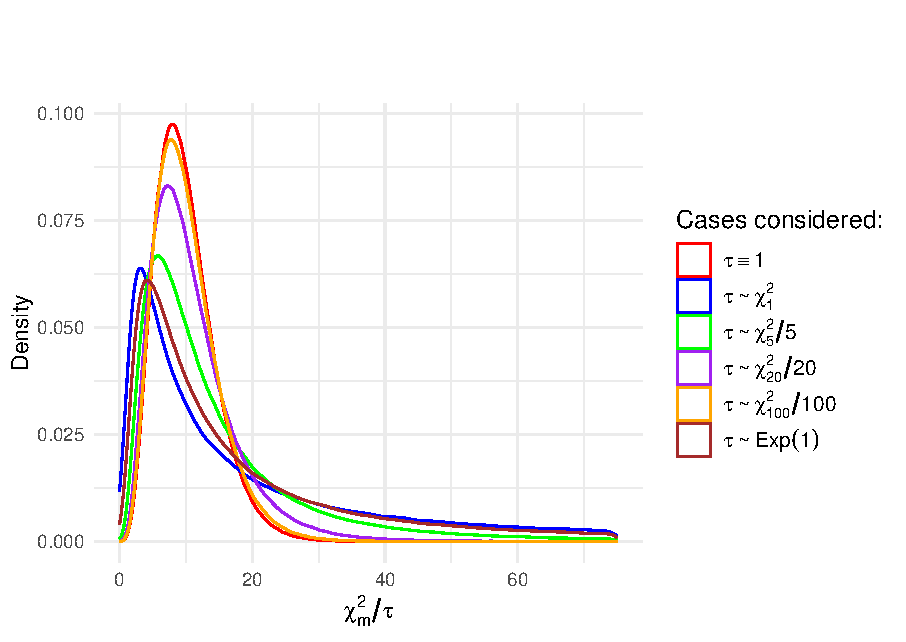
\includegraphics[scale=.7]{pics/SNMtails.pdf}
	\end{center}
\end{frame}

\begin{frame}{}
Some tails are \alert{much} heavier than Gaussian. \\[3mm]

In the plot above we study $Y=\|X-\mu\|_\Sigma^2$ for $X$: normal, multivariate t, Laplace. 
	\begin{table}[h]
    \centering
    \begin{tabular}{lcccc}
        \hline
        \textbf{Case} & $P(Y > 75)$ & $P(Y > 500)$ & $P(Y > 1000)$ & $P(Y > 10000)$ \\
        \hline
        Gaussian & 0.000 & 0.000 & 0.000 & 0.000 \\
        $t_{100}$ & 0.000 & 0.000 & 0.000 & 0.000 \\
        $t_{20}$ & 0.000 & 0.000 & 0.000 & 0.000 \\
        $t_{5}$ & 0.019 & 0.000 & 0.000 & 0.000 \\
        Laplace & 0.124 & 0.020 & 0.010 & 0.001 \\
        $t_{1}$ & 0.277 & 0.109 & 0.077 & 0.024 \\
        \hline
    \end{tabular}
    \caption{Proportion of Samples Exceeding Thresholds}
    \label{tab:proportion_thresholds}
\end{table}
\end{frame}

\begin{frame}[fragile]{Simple illustration}
In the notes we provide an example of four stocks: Apple, Microsoft, Google, Amazon.\\[3mm]
Compare the empirical distribution of the Mahalanobis distance with $\chi^2_4$ (Gaussian).\\[3mm]
\begin{minipage}{7cm}
	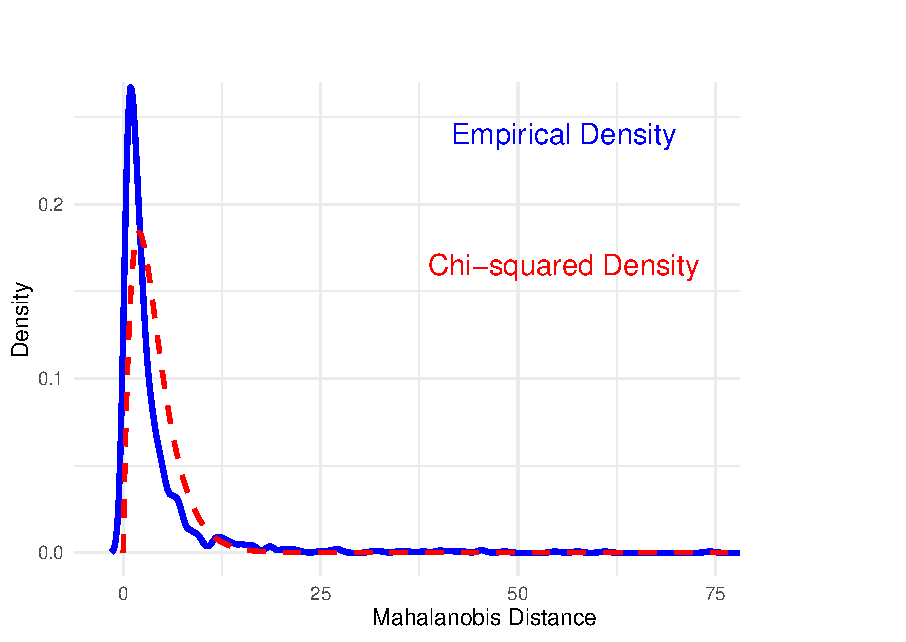
\includegraphics[scale=.5]{pics/SMN2.pdf}
\end{minipage}\begin{minipage}{8cm}
	Empirical density seems to be more concentrated around zero.\\[3mm]
	But it has much heavier tails. 
	\begin{itemize}
		\item $\P(\chi^2_4>20)\approx 0$. 
		\item $\P(Y>20)\approx 0.03$
	\end{itemize}
\end{minipage}
\smallskip

This may be much more dramatic for smaller companies.
\end{frame}



\section{Copula models}

\begin{frame}{}
	\begin{center}
		{\Huge \alert{Copula models}}
	\end{center}
\end{frame}

\begin{frame}{Cumulative Distribution Function (CDF)}
	Let $X=(X_1,\ldots,X_m)$ be a random vector.  Its \textbf{CDF} is: $$F(x_1,\ldots,x_m)=\P(X_1\leq x_1,X_2\leq x_2,\ldots,X_m\leq x_m).$$
	Marginal CDF: $F_1(x_1)=\P(X_1\leq x_1)=\lim_{x_2\to \infty}\cdots\lim_{x_m\to\infty}F(x_1,x_2,\ldots,x_m)$.
	(similar for any other margin)\\[5mm]	
	\begin{block}{}
	If $f$ is the corresponding density of $X$, then:
	$$
	f(x_1,\ldots,x_m)\;=\;\frac{\partial^m}{\partial x_1\cdots\partial x_m}F(x_1,\ldots,x_m)
	$$
	
	$$
	F(x_1,\ldots,x_m)\;=\;\int_{-\infty}^{x_1}\cdots \int_{-\infty}^{x_m} f(y_1,\ldots,y_m){\rm d}y_1\cdots {\rm d} y_m. 
	$$		
	\end{block}
		If $U\sim U[0,1]$ then $F(u)=u$ for all $u\in [0,1]$.

\end{frame}


\begin{frame}{What is a Copula?}
\begin{itemize}
    \item A \textbf{copula} is a function that captures the \textbf{dependence structure} between random variables, separate from their marginal distributions.
\end{itemize}
\begin{alertblock}{Definition}
	A function $C : [0, 1]^m \to [0, 1]$ is a \textbf{copula} if it is a CDF with uniform marginals, that is, $C_1(u_1)=u_1$, \ldots, $C_m(u_m)=u_m$, where $C_i$ are the marginal CDF's.
\end{alertblock}
For example, the copula $C(\bs u)=u_1\cdots u_m$ corresponds to a $m$ independent $U[0,1]$.
\begin{block}{Why use copulas?}
	\begin{itemize}
        \item To model non-Gaussian dependencies.
        \item To analyze dependence independently of marginal behaviors.
    \end{itemize}
\end{block}
\end{frame}

% Slide 2: Sklar's Theorem
\begin{frame}{Sklar's Theorem}
\begin{block}{Theorem (Sklar, 1959)}
Let $X = (X_1, \ldots, X_m)$ be a \textbf{continuous} random vector with joint CDF $F$ and marginals $F_1, \ldots, F_m$. There exists a unique copula $C$ such that:
\begin{equation}\label{eq:copula}
	F(x_1, \dots, x_m) = C(F_1(x_1), \dots, F_m(x_m)). 
\end{equation}
Conversely, given marginals $F_1, \ldots, F_m$ and a copula $C$, $F$ in \eqref{eq:copula} is a CDF of a multivariate distribution with given margins.
\end{block}
\begin{itemize}
    \item $C$ captures \textbf{dependence structure}.
    \item $F_1, \ldots, F_m$ capture marginal behaviors.
\end{itemize}
\end{frame}

% Slide 3: Understanding Sklar's Theorem
\begin{frame}{Understanding Sklar's Theorem}
%    \item When $m = 1$, $C(u) = u$, the identity function on $[0, 1]$.\\[5mm]
\begin{alertblock}{}
If $X$ is continuous with CDF $F$, then $F(X) \sim U(0, 1)$. 	
\end{alertblock}
    \textbf{Proof:} If $X$ is continuous, $F$ is strictly increasing on the support. Hence
    \[
    \mathbb{P}(F(X) \leq u) = \mathbb{P}(X \leq F^{-1}(u)) = F(F^{-1}(u)) = u.
    \]
    \vspace{-7mm}
\begin{block}{}
	Let $X = (X_1, \ldots, X_m)$ with CDF $F$ and margins $F_i$. Define $U_i := F_i(X_i)$.
	\begin{itemize}
		\item The transformed variables $U = (U_1, \ldots, U_m)$ have uniform marginals.
    \[ \mathbb{P}(U_1 \leq u_1, \ldots, U_m \leq u_m) =: C(u_1, \ldots, u_m). \]
    \item Also $C(\bs u)$ is given explicitly in terms of $F$ and $F_i$'s:
    \begin{equation}\label{eq:cop1}
    C(\bs u)=\mathbb{P}(F_1(X_1) \leq u_1, \ldots, F_m(X_m) \leq u_m) = F(F_1^{-1}(u_1),\ldots,F_m^{-1}(u_m))	
\end{equation}
	\end{itemize}
\end{block}
\end{frame}

% Slide 5: Example of a Copula
\begin{frame}{Simple Example of a Copula}
\begin{itemize}
    \item Joint CDF:
    \[ F_{X,Y}(x, y) =
    \begin{cases} 
    0 & x < 0 \text{ or } y < 0, \\
    x^2 y^2 & 0 \leq x, y \leq 1, \\
    1 & x > 1 \text{ and } y > 1, \\
    \min(x^2, y^2) & \text{otherwise}.
    \end{cases} \]
    \item Marginal CDFs:
    \[ F_X(x) = x^2, \quad F_Y(y) = y^2 \quad \text{for } 0 \leq x, y \leq 1. \]
    \item Copula:
    \[ C(u, v) = uv \quad \text{if } u, v \leq 1. \]
\end{itemize}
\end{frame}


\begin{frame}{Sampling}
	Fix a copula $C(\bs u)$ and suppose we can sample from it.
	\begin{block}{Transform the copula sample}
		Consider a sample $\bs u^{(1)}$, \ldots, $\bs u^{(n)}$ from the copula.\\[3mm]
		
		Transform the data to have the right marginals $F_1,\ldots,F_m$:
		$$
		\x^{(t)}_i \;:=\; F_i^{-1}(\bs u^{(t)}_i)\qquad\mbox{for all }i=1,\ldots,m, t=1,\ldots,n.
		$$
		The sample $\x^{(1)},\ldots,\x^{(n)}$ has the right marginals and the right dependence structure. 
		$$
		\P(\x_i^{(t)}\leq s_i)=\P(F_i^{-1}(\bs u_i^{(t)})\leq s_i)=\P(\bs u_i^{(t)}\leq F_i(s_i))=F_i(s_i).
		$$
	\end{block}
	\medskip
	We will later show how to sample from some popular copula models. 
\end{frame}


% Slide 6: Invariance under Transformations
\begin{frame}{Invariance under Monotone Transformations}
\begin{alertblock}{Copulas are invariant under monotone transformations. }
	Consider $Y_i := f_i(X_i)$, where $f_i$ are strictly increasing transformations. Then the copula of $X$ is the same as the copula of $Y$. 
\end{alertblock}
Proof: Let $G$ be the CDF of $Y$ and $G_i$ the marginal CDF of $Y_i$
    \begin{itemize}
    \item By \eqref{eq:cop1}, equiv. show $F(F_1^{-1}(u_1), \ldots, F_m^{-1}(u_m))=G(G_1^{-1}(u_1), \ldots, G_m^{-1}(u_m))$
        \item $G_i(y_i)=\P(Y_i\leq y_i)=\P(f_i(X_i)\leq y_i)=\P(X_i\leq f_i^{-1}(y_i))=F_i(f_i^{-1}(y_i))$.
        \item Thus, $\{Y_i\leq G_i^{-1}(u_i)\}=\{F_i(f_i^{-1}(Y_i))\leq u_i\}=\{F_i(X_i)\leq u_i\}=\{X_i\leq F^{-1}_i(u_i)\}$ and so  
      \begin{eqnarray*}
      	&&G(G_1^{-1}(u_1),\ldots, G_m^{-1}(u_m))= \P\left(\bigcap_{i=1}^m \{Y_i\leq G^{-1}_i(u_i)\}\right)\\
      	&=&\P\left(\bigcap_{i=1}^m \{X_i\leq F^{-1}_i(u_i)\}\right)=F(F_1^{-1}(u_1), \ldots, F_m^{-1}(u_m)).
      \end{eqnarray*} 
    \end{itemize}
\end{frame}

% Slide 7: Copula Density
\begin{frame}{Density of a Copula}
The PDF of a copula $C$ is obtained by differentiating its CDF:
    \[ c(\mathbf{u}) = \frac{\partial^m C(\mathbf{u})}{\partial u_1 \cdots \partial u_m}. \]
    
    Recall $C(\bs u)=F(F_1^{-1}(u_1),\ldots, F_m^{-1}(u_m))$. By chain rule and inverse function theorem:
    \[ c(\mathbf{u}) = \frac{f(\mathbf{x})}{\prod_{i=1}^m f_i(x_i)},\qquad \mbox{where } x_i=F_i^{-1}(u_i)\mbox{ for all }i \]
    where $f$ is the joint density and $f_i$ are marginal densities.
    \bigskip
    
    e.g. $C(\bs u)=u_1\cdots u_m$ is the CDF of independent $U_i\sim U(0,1)$. The density is uniform on $[0,1]^m$. Given margins $f_i$, we get $f(\x)=\prod_i f_i(x_i)$.
\end{frame}

% Slide 8: Gaussian Copula
\begin{frame}{Gaussian Copula}
Gaussian copula is derived from the multivariate normal distribution $X\sim N_m(\mu,\Sigma)$.\\[3mm]
By monotone invariance, we can assume $\E X_i=0$, $\var(X_i)=1$
\begin{itemize}
	\item  $\mu=0$, $\Sigma$ is a correlation matrix,
	\item each $X_i\sim N(0,1)$. 
\end{itemize}
 

Let $\Phi$ be the CDF of $N(0,1)$ with PDF $\phi$. Let $f(\x;\Sigma)$ be the PDF of $N_m(\bs 0,\Sigma)$.
\begin{alertblock}{The density of the Gaussian copula $C(\bs u;\Sigma)$}
	Using the general formula, we get:
	\[ c(\mathbf{u}; \Sigma) \;=\; \frac{f(\x;\Sigma)}{\prod_{i=1}^m \phi(x_i)}\;=\; \det(\Sigma)^{-1/2} \exp\left(-\frac{1}{2} \mathbf{x}^\top (\Sigma^{-1} - I_m) \mathbf{x}\right), \]
	where $\x=(\Phi^{-1}(u_1),\ldots,\Phi^{-1}(u_m))$.
\end{alertblock}
 \end{frame}

\begin{frame}{Sampling from the Gaussian copula $C(\bs u;\Sigma)$}
Let $\Sigma$ be a correlation matrix.\\[3mm]
\begin{itemize}
	\item Sample $\z^{(1)},\ldots,\z^{(n)}\sim N_m(\bs 0,\Sigma)$.\\[3mm]
	\item Transform $\bs u^{(t)}_i=\Phi(\z^{(t)}_i)$ for all $i=1,\ldots,m$ and $t=1,\ldots,n$. \\[3mm]
	\item The sample $\bs u^{(1)},\ldots,\bs u^{(n)}$ comes from the Gaussian copula. \\[3mm]
\end{itemize}	
	As described earlier, we can now transform this sample to get arbitrary margins.\\[3mm]
	\begin{block}{}
		The Gaussian copula model can still handle quite general distributions. Yet, it retains some of the computational advantages of the Gaussian distribution.
	\end{block}

\end{frame}

\begin{frame}{Steps to Estimate a Copula: normalize data}
	Given data $\x^{(1)},\ldots,\x^{(n)}$, start by fixing a copula model (e.g. Gaussian).\\[3mm]
	
	We assume the CDF $F$ of the data satisfies $F(\x)=C(F_1(x_1),\ldots,F_m(x_m))$.\\[3mm]
	
	However, \alert{the margins $F_i$ are not known!}\\[3mm]
	
	Given a sample $\x_i^{(1)},\ldots,\x_i^{(n)}$ of $X_i$ we compute the \textbf{empirical CDF} (proxy for $F_i$)
	$$
	\widehat F_i(x_i)\;:=\;\frac1n \sum_{t=1}^n \bs 1\{\x_i^{(t)}\leq x_i\}\;\approx\;\P(X_i\leq x_i)\;=\;F_i(x_i).
	$$
	\vspace{-5mm}
\begin{alertblock}{}
	Transform, each row in the data matrix $\X$ using the empirical CDFs
$$
\bs u^{(t)}_i\;=\;\widehat F_i(\x^{(t)}_i)\quad\mbox{for } i=1,\ldots,m.
$$
The transformed data matrix $\bs U$ contains samples coming from $U(0,1)$.
\end{alertblock}\end{frame}


\begin{frame}{Steps to Estimate a Copula: Fit the copula family}
Previous slide: \;\;$\x^{(t)}\to \bs u^{(t)}$ using the empirical CDFs.\\[5mm]
In the next step, we fit the data to the given copula family. \\[3mm]

Often this is done by maximizing the log-likelihood $\sum_{t=1}^n \log c(\bs u^{(t)})$.
\begin{block}{The Gaussian copula case $C(\bs u;\Sigma)$}
	The goal is to estimate $\Sigma$ based on the likelihood. 
\begin{itemize}
	\item Transform the data to standard Gaussian margins: $\y^{(t)}_i=\Phi^{-1}(\bs u^{(t)}_i)$.
	\item Fit the Gaussian likelihood for $N_m(\bs 0,\Sigma)$ with the sample covariance  $S_n=\tfrac1n \Y^\top \Y$.
\end{itemize}	
\end{block}
\end{frame}


\begin{frame}{Steps to Estimate a Copula: Evaluate the fit}
As the last step, compare the fitted copula model with the observed data. Check whether the copula captures the dependence structure accurately.\\[3mm]
We can generate samples from the fitted Gaussian copula.
\end{frame}




%% Slide 9: Applications of Copulas
%\begin{frame}{Applications of Copulas}
%\begin{itemize}
%    \item \textbf{Finance:} Modeling dependencies in asset returns.
%    \item \textbf{Insurance:} Understanding risks in correlated claims.
%    \item \textbf{Environmental Science:} Joint modeling of extreme events (e.g., floods).
%    \item \textbf{Medical Statistics:} Modeling dependence in survival times.
%\end{itemize}
%\end{frame}

\begin{frame}{Simulating Realistic Financial Portfolios with Gaussian Copulas}
	\textbf{Goal:}
Use Gaussian copulas to model and generate synthetic financial returns that preserve real-world dependencies but remain flexible in capturing tail dependencies. This method is widely used in risk management, portfolio optimization, and even in synthetic data generation for AI models in finance.
\begin{itemize}
	\item After fitting a copula model simulate synthetic data from it.
	\item Apply the inverse transformations to get to the original scale: $X_i^{\text{new}} = F_i^{-1}(U_i^{\text{sim}})$
\end{itemize}
This creates synthetic but realistic asset returns that match observed dependencies!
\begin{block}{Applications:}
\begin{itemize}
	\item Stress Testing \& Risk Management
	\item Portfolio Optimization
	\item Synthetic Data for AI Models
\end{itemize}
\end{block}
\end{frame}

\section{Gaussian mixture models}

\begin{frame}{}
	\begin{center}
		{\Huge \alert{Gaussian mixtures}}
	\end{center}
\end{frame}


% Slide 1: Definition of GMMs
\begin{frame}{Mixture of Gaussians}
We combine simple models into a complex model by taking a mixture of $K$ multivariate Gaussian densities of the form:
$$
p(x)\;=\;\sum_{k=1}^K \pi_k N_m(x|\mu_k,\Sigma_k)\quad\mbox{for }x\in \R^m,
$$
where $\pi_k\geq 0$, $\sum_{k=1}^K\pi_k=1$, and $N_m(x|\mu_k,\Sigma_k)$ is the $m$-dim Gaussian density.
\begin{itemize}
	\item Each Gaussian component has its own mean vector $\mu_k$ and covariance matrix $\Sigma_k$.
	\item The parameters $\pi_k$ are called the mixing coefficients.
\end{itemize}
\pause
\begin{minipage}{7cm}{}
Example:
\begin{itemize}
	\item $K=3$ (three Gaussian components)
	\item $m=1$ (univariate Gaussians)
\end{itemize}
\end{minipage}\begin{minipage}{5cm}{}
	\begin{figure}
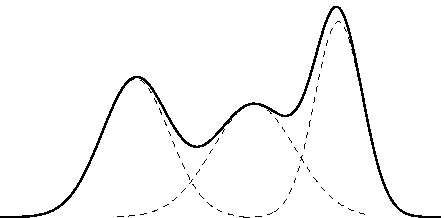
\includegraphics[scale=.25]{./pics/multimodal.jpg}
\end{figure}
\end{minipage}
\end{frame}

\begin{frame}{The crabs from Naples bay}

%	{In 1892, scientists collected data on populations of the crab and observed that the ratio of forehead width to the body length  actually showed a highly skewed distribution.}\\[.2cm]

%	\begin{figure*}
\begin{minipage}{5.5cm}{}
	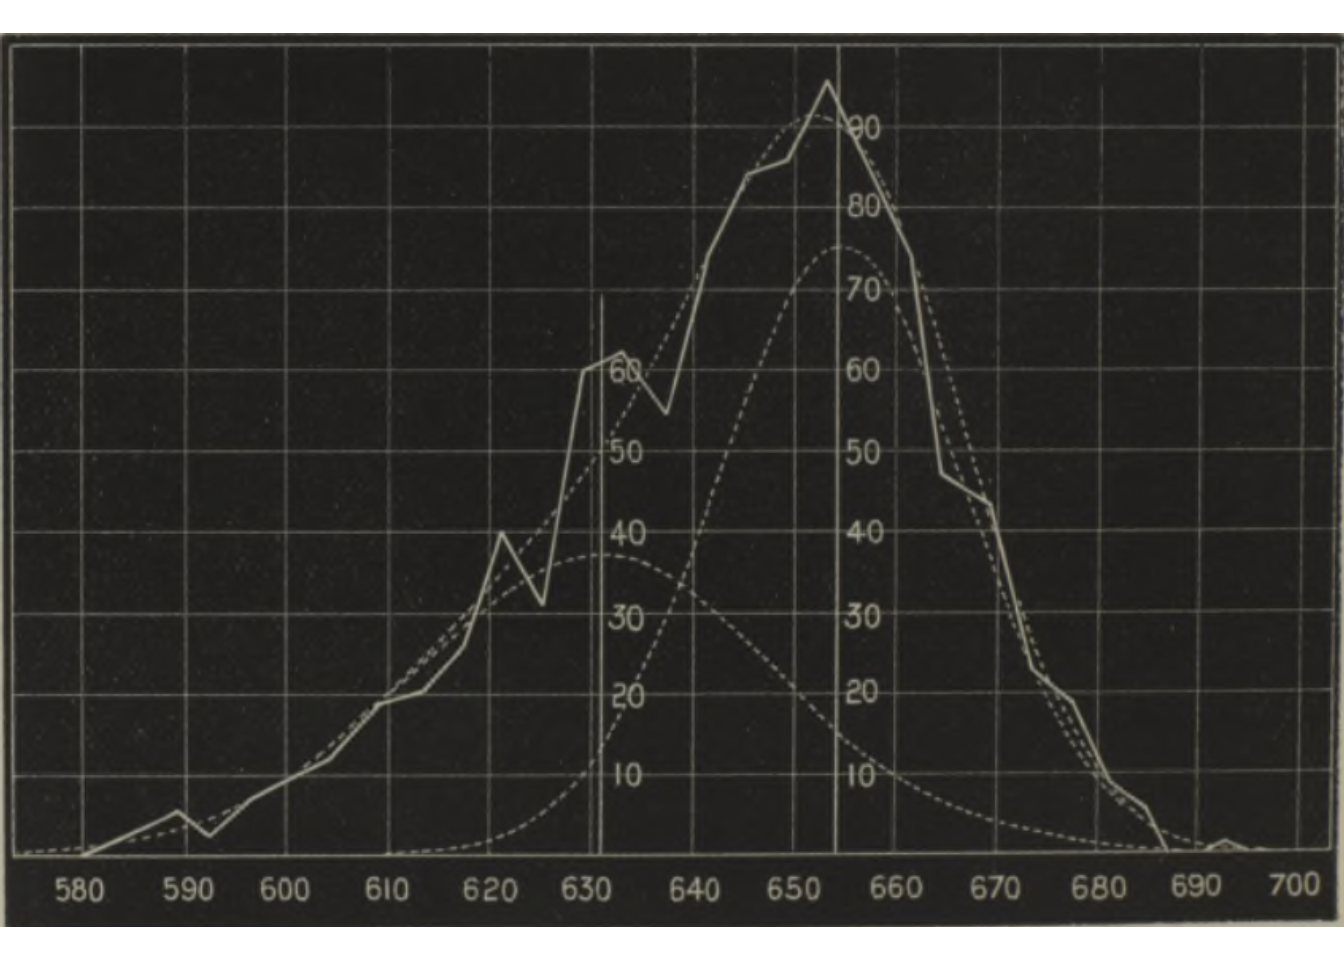
\includegraphics[scale=.29]{pics/crabs.png}
		\end{minipage}\begin{minipage}{9cm}
			 In 1892, scientists collected data on populations of the crab and observed that the ratio of forehead width to the body length  actually showed a highly skewed distribution.\\[2mm] {\small Source: \textit{On Certain Correlated Variations in Carcinus maenas} (1893) W. F.  Weldon.}	
		\end{minipage}

{ They wondered whether this distribution could be the result of the population being a mix of two different normal distributions (two sub-species).}
\smallskip 

{ In \textbf{1894}, Karl Pearson proposed a method to fit this model (\href{https://archive.org/details/philtrans02543681}{\textcolor{blue}{read here}}), whose modern version is the ``method of moments''. The method involved solving a higher order polynomial.}
%	\end{figure*}
\end{frame}

\begin{frame}{Mixture of Gaussians: 2D example}
Illustration of a mixture of three Gaussians in 2D.
\begin{figure}
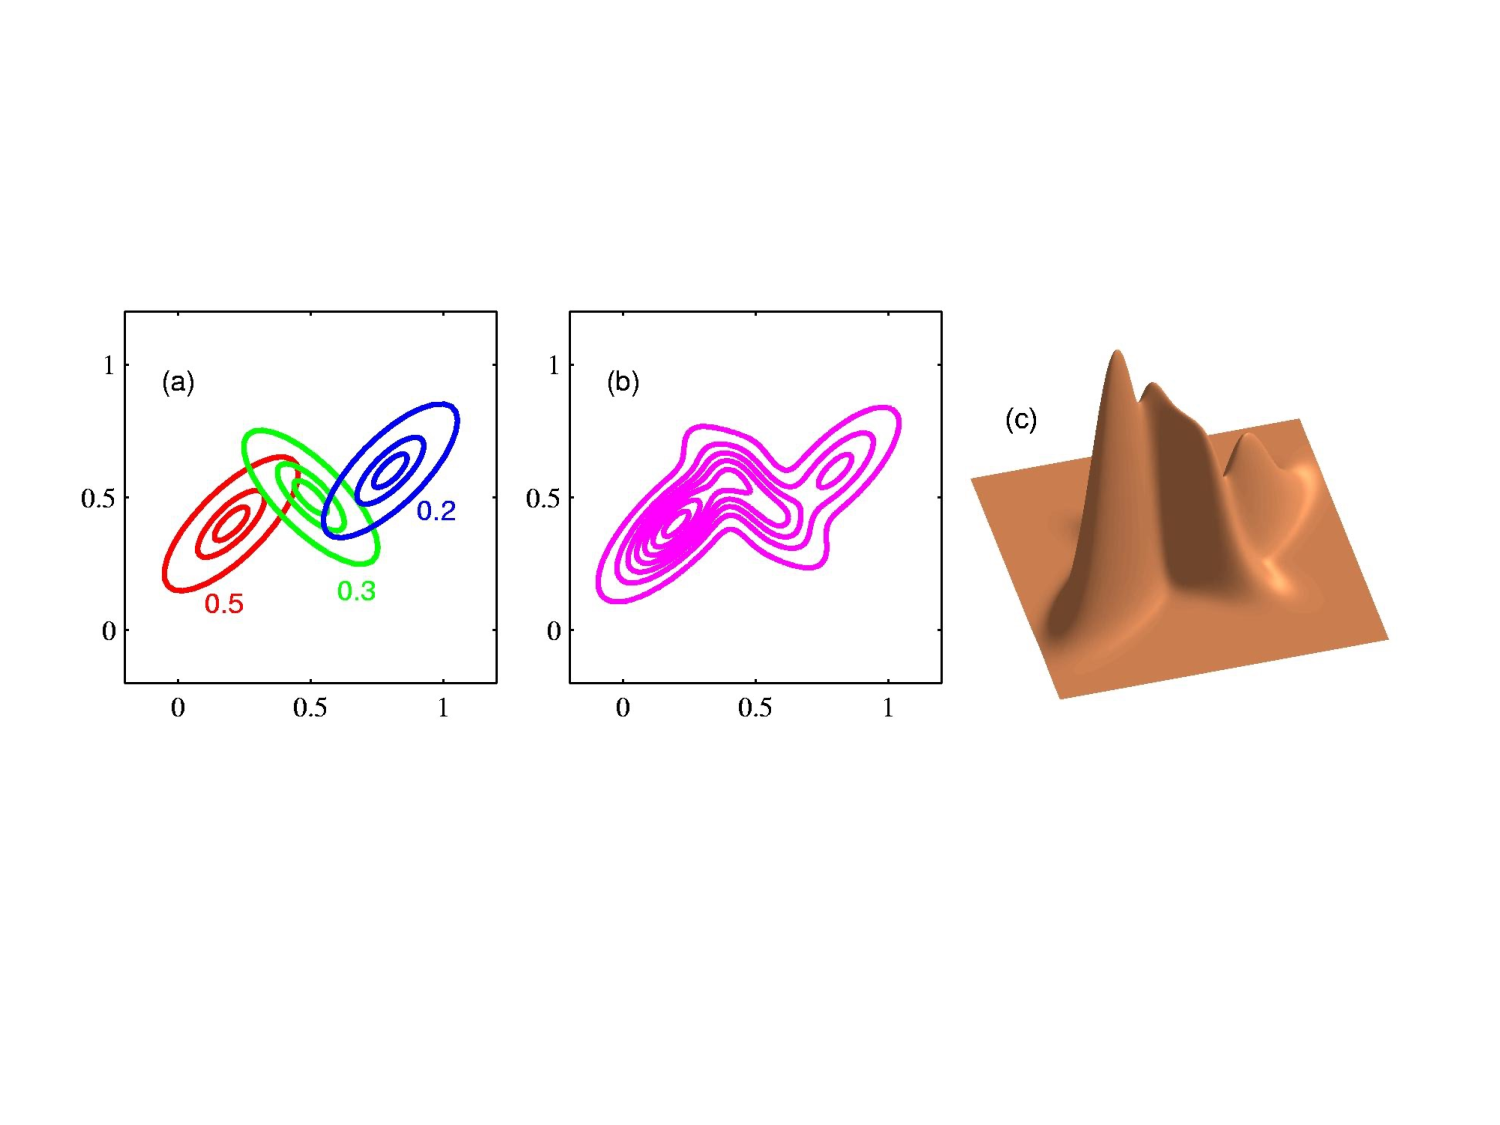
\includegraphics[width=4.8in]{pics/raw1.pdf}
\end{figure}
\vspace{-5mm}
\begin{itemize}
	\item [(a)] Contours of constant density of each of the mixture components, along with the mixing coefficients. 
	\item [(b)] Contours of marginal density $p(\x)=\sum_{k=1}^K \pi_k N_m(\x|\mu_k,\Sigma_k)$.
	\item [(c)] A surface plot of the distribution $p(\x)$.
\end{itemize}
\end{frame}

% Slide 2: Why use Gaussian Mixtures?
\begin{frame}{Why Use Gaussian Mixtures?}
Gaussian Mixture Models (GMMs) are widely used because of their:
\begin{itemize}
    \item \textbf{Flexibility:} Ability to model complex data distributions.
    \item \textbf{Multimodality:} Handles datasets with multiple clusters or modes.
    \item \textbf{Interpretability:} Each Gaussian component represents a sub-population with interpretable parameters.
    \item \textbf{Clustering Applications:} GMMs are a natural probabilistic method for clustering.
\end{itemize}

\textbf{Special Case:}
For simplicity, in clustering, we often assume \( \Sigma_k = \Sigma \) for all \( k \).
\end{frame}

\begin{frame}
\frametitle{Mixture of Gaussians as a latent variable model}
Recall: \textcolor{blue}{$p(x)\;=\;\sum_{k=1}^K \pi_k N_m(x|\mu_k,\Sigma_k)$}.\\[.3cm]
\begin{itemize}
	\item Consider a latent variable $z$ with $K$ states $z\in \{1,\ldots,K\}$. 
%	\item For simplicity encode it in a 1-to-K representation:
%	$$
%	z\in \{e_1,\ldots,e_K\},\quad  \mbox{where } e_i=(0,\ldots,0,1,0,\ldots,0).
%	$$
	\item The distribution of $z$ given by the mixing coefficients: $$p(z=k)=\pi_k.$$
	\item Specify the conditional as $p(x|z=k)=N_m(x|\mu_k,\Sigma_k)$ with joint: $$p(x,z=k)\;=\;p(z=k)p(x|z=k)\;=\;\pi_k N_m(x|\mu_k,\Sigma_k).$$
	\item Then the marginal $p(x)$ satisfies $$\textcolor{blue}{p(x)=\sum_{k=1}^K p(x,z=k)\;=\;\sum_{k=1}^K \pi_k N_m(x|\mu_k,\Sigma_k)}.$$
\end{itemize}
%\begin{figure}
%\includegraphics[page=3,width=4.8in,trim={0 0 0 3cm},clip]{./raw.pdf}
%\end{figure}
\end{frame}

\begin{frame}{Yet another illustration}
The quantities $p(z|x)$ are called responsibilities.\\[3mm]
Consider 500 points drawn from a mixture of three Gaussians. 
\begin{figure}
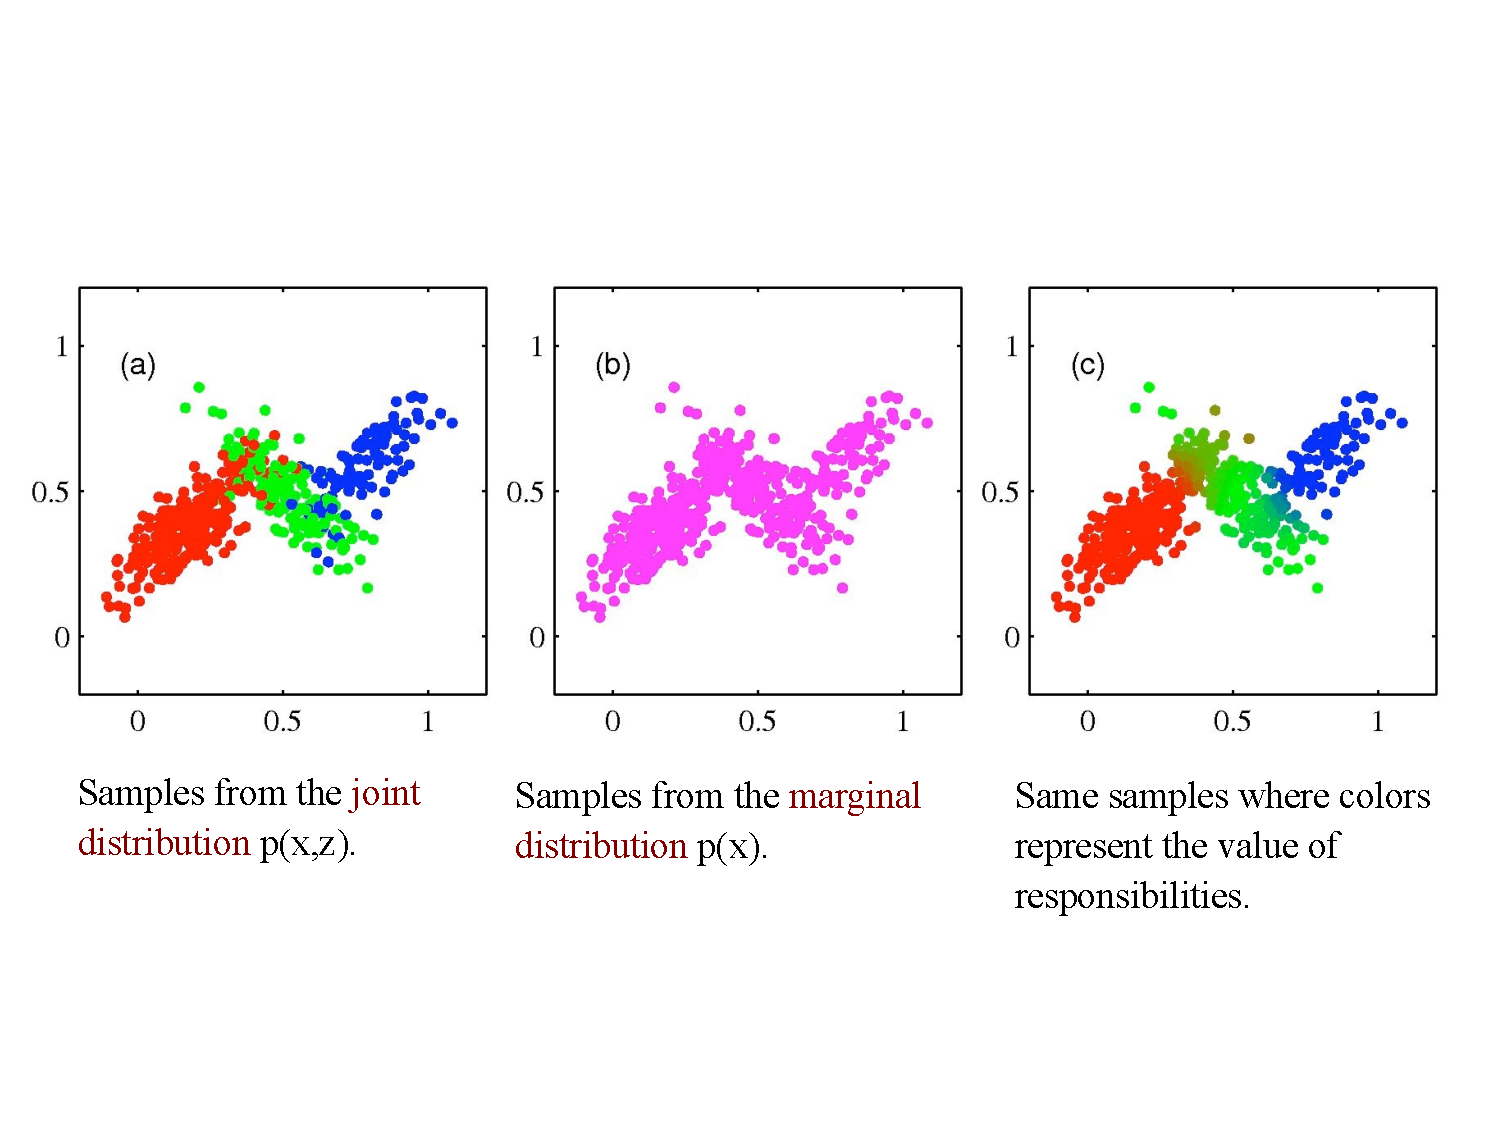
\includegraphics[width=4.8in]{pics/raw2.pdf}
\end{figure}
\end{frame}

\begin{frame}{The Likelihood function}
Parameters: $\boldsymbol\pi=(\pi_1,\ldots,\pi_K)$, $\boldsymbol\mu=(\mu_1,\ldots,\mu_K)$, $\boldsymbol\Sigma=(\Sigma_1,\ldots,\Sigma_K)$.

Recall: $\textcolor{blue}{p(x|\boldsymbol\pi,\boldsymbol\mu,\boldsymbol\Sigma)=\sum_{k=1}^K \pi_k N_m(x|\mu_k,\Sigma_k)}$
\medskip

\begin{itemize}
	\item Represent the dataset $\{x_1,\ldots,x_N\}$ as $\boldsymbol X\in \mathbb R^{N\times m}$.
	\item The latent variable is represented by a vector $\boldsymbol z\in \mathbb R^N$.
	\item The log-likelihood takes the form $$\log p(\boldsymbol X|\boldsymbol\pi,\boldsymbol\mu,\boldsymbol\Sigma)=\sum_{n=1}^N\log\left(\sum_{k=1}^K\pi_k N_m(x_n|\mu_k,\Sigma_k)\right)$$
\end{itemize}
%\begin{figure}
%\includegraphics[page=9,width=1.8in,trim={16.5cm 3.5cm 0cm 8cm},clip]{./raw.pdf}
%\end{figure}
\end{frame}

\begin{frame}{Maximum Likelihood ($\boldsymbol \mu$)}
Recall: $\log p(\boldsymbol X|\boldsymbol\pi,\boldsymbol\mu,\boldsymbol\Sigma)=\sum_{n=1}^N\log\left(\sum_{k=1}^K\pi_k N_m(x_n|\mu_k,\Sigma_k)\right)$.
\begin{itemize}
%	\item The log-likelihood takes the form $$\log p(\boldsymbol X|\boldsymbol\pi,\boldsymbol\mu,\boldsymbol\Sigma)=\sum_{n=1}^N\log\left(\sum_{k=1}^K\pi_k N_m(x_n|\mu_k,\Sigma_k)\right)$$
	\item Differentiating wrt $\mu_k$ and setting to zero gives:
	\begin{eqnarray*}
		0&=&\sum_{n=1}^N\frac{\pi_k N(x_n|\mu_k,\Sigma_k)}{\sum_j \pi_j N(x_n|\mu_j,\Sigma_j)}\Sigma_k^{-1}(x_n-\mu_k)\;=\; \sum_{n=1}^N p(z_n=k|x_n)\Sigma_k^{-1}(x_n-\mu_k)\\[2mm]\pause
		&=&\Sigma_k^{-1}\left(\sum_{n=1}^N p(z_n=k|x_n)x_n-\mu_k\textcolor{red!80!green!20!blue}{\sum_{n=1}^N p(z_n=k|x_n)}\right).
	\end{eqnarray*} 	
	\item Equivalently (as $\Sigma_k$ is positive definite) $$\mu_k\;=\;\sum_n \frac{p(z=k|x_n)}{N_k}x_n,\qquad N_k=\textcolor{red!80!green!20!blue}{\sum_n p(z=k|x_n)}.$$
	\item Simple interpretation: the MLE given by the weighted mean of the data weighted by the posterior $p(z=k|x_n)$.
\end{itemize}
%\begin{figure}
%\includegraphics[page=9,width=1.8in,trim={16.5cm 3.5cm 0cm 8cm},clip]{./raw.pdf}
%\end{figure}
\end{frame}



%\begin{frame}
%\frametitle{Maximum Likelihood}
%\begin{figure}
%\includegraphics[page=10,width=4.8in,trim={0 0 0 3cm},clip]{./raw.pdf}
%\end{figure}
%\end{frame}

%\begin{frame}
%\frametitle{Maximum Likelihood}
%\begin{figure}
%\includegraphics[page=11,width=4.8in,trim={0 0 0 3cm},clip]{./raw.pdf}
%\end{figure}
%\end{frame}

\begin{frame}{Maximum Likelihood ($\boldsymbol \Sigma,\boldsymbol \pi$)}
Recall: $\log p(\boldsymbol X|\boldsymbol\pi,\boldsymbol\mu,\boldsymbol\Sigma)=\sum_{n=1}^N\log\left(\sum_{k=1}^K\pi_k N_m(x_n|\mu_k,\Sigma_k)\right)$.
\begin{itemize}
	\item Differentiating wrt $\Sigma_k$ and setting to zero gives:
	$$\Sigma_k\;=\;\sum_n \frac{p(z=k|x_n)}{N_k}(x_n-\mu_k)(x_n-\mu_k)^\top.$$
	\item Again data points weighted by posterior probabilities.\\[.4cm]
	\item Finally, for the weights $\pi_k$ the MLE is
$$
\pi_k\;=\;\frac{N_k}{\sum_{j=1}^K N_j}\;=\;\frac{N_k}{N},\qquad N_k=\sum_n p(z=k|x_n).
$$
\end{itemize}
%\begin{figure}
%\includegraphics[page=9,width=1.8in,trim={16.5cm 3.5cm 0cm 8cm},clip]{./raw.pdf}
%\end{figure}
\end{frame}


%\begin{frame}
%\frametitle{Maximum Likelihood}
%\begin{figure}
%\includegraphics[page=12,width=4.8in,trim={0 0 0 3cm},clip]{./raw.pdf}
%\end{figure}
%\end{frame}

%\begin{frame}
%\frametitle{Maximum Likelihood}
%\begin{figure}
%\includegraphics[page=13,width=4.8in,trim={0 0 0 3cm},clip]{./raw.pdf}
%\end{figure}
%\end{frame}

\begin{frame}{Motivating the EM algorithm}
\begin{itemize}
	\item The MLE \textcolor{red}{does not have a closed form solution.}
	\item The estimates depend on the posterior probabilities $p(z=k|x_n)$, which themselves depend on those parameters.
	\item Indeed, recall that $$p(z=k|x_n)\;=\;\frac{\pi_k N_m(x_n|\mu_k,\Sigma_k)}{\sum_{j=1}^K \pi_j N_m(x_n|\mu_j,\Sigma_j)}.
$$
\item Iterative solution (EM algorithm):
\begin{itemize}
\item Initialize the parameters to some values.
\item [\textcolor{red}{E-step}] Update the posteriors $p(z=k|x_n)$.
\item [\textcolor{red}{M-step}] Update model parameters $\boldsymbol\pi,\boldsymbol\mu,\boldsymbol\Sigma$.
\item Repeat.
\end{itemize}
\end{itemize}
%\begin{figure}
%\includegraphics[page=14,width=4.8in,trim={0 0 0 3cm},clip]{./raw.pdf}
%\end{figure}
\end{frame}

%\begin{frame}
%\frametitle{Maximum Likelihood}
%\begin{figure}
%\includegraphics[page=15,width=4.8in,trim={0 0 0 3cm},clip]{./raw.pdf}
%\end{figure}
%\end{frame}

\begin{frame}[label=GMEM]{EM algorithm for Gaussian mixtures}
	\begin{itemize}
		\item Initialize $\boldsymbol\pi,\boldsymbol\mu,\boldsymbol\Sigma$.
		\item \textcolor{red}{E-step}: for each $k,n$ compute the posterior probabilities $$p(z=k|x_n)\;=\;\frac{\pi_k N_m(x_n|\mu_k,\Sigma_k)}{\sum_{j=1}^K \pi_j N_m(x_n|\mu_j,\Sigma_j)}.$$
		\item \textcolor{red}{M-step}: Re-estimate model parameters
		\begin{align*}
			\mu_k^{\rm new} & =\sum_{n=1}^N \frac{p(z=k|x_n)}{N_k}x_n,\qquad N_k=\sum_{n=1}^N p(z=k|x_n),\\
			\Sigma_k^{\rm new} & = \sum_{n=1}^N \frac{p(z=k|x_n)}{N_k}(x_n-\mu_k^{\rm new})(x_n-\mu_k^{\rm new})^\top,\\
			\pi_k^{\rm new} & = \frac{N_k}{N}.
		\end{align*}
		\item Evaluate the log-likelihood and check for convergence. 
	\end{itemize}
\end{frame}

%\begin{frame}
%\frametitle{EM algorithm}
%\begin{figure}
%\includegraphics[page=16,width=4.8in,trim={0 0 0 3cm},clip]{./raw.pdf}
%\end{figure}
%\end{frame}

\begin{frame}{Visualization of EM Algorithm}
\begin{figure}
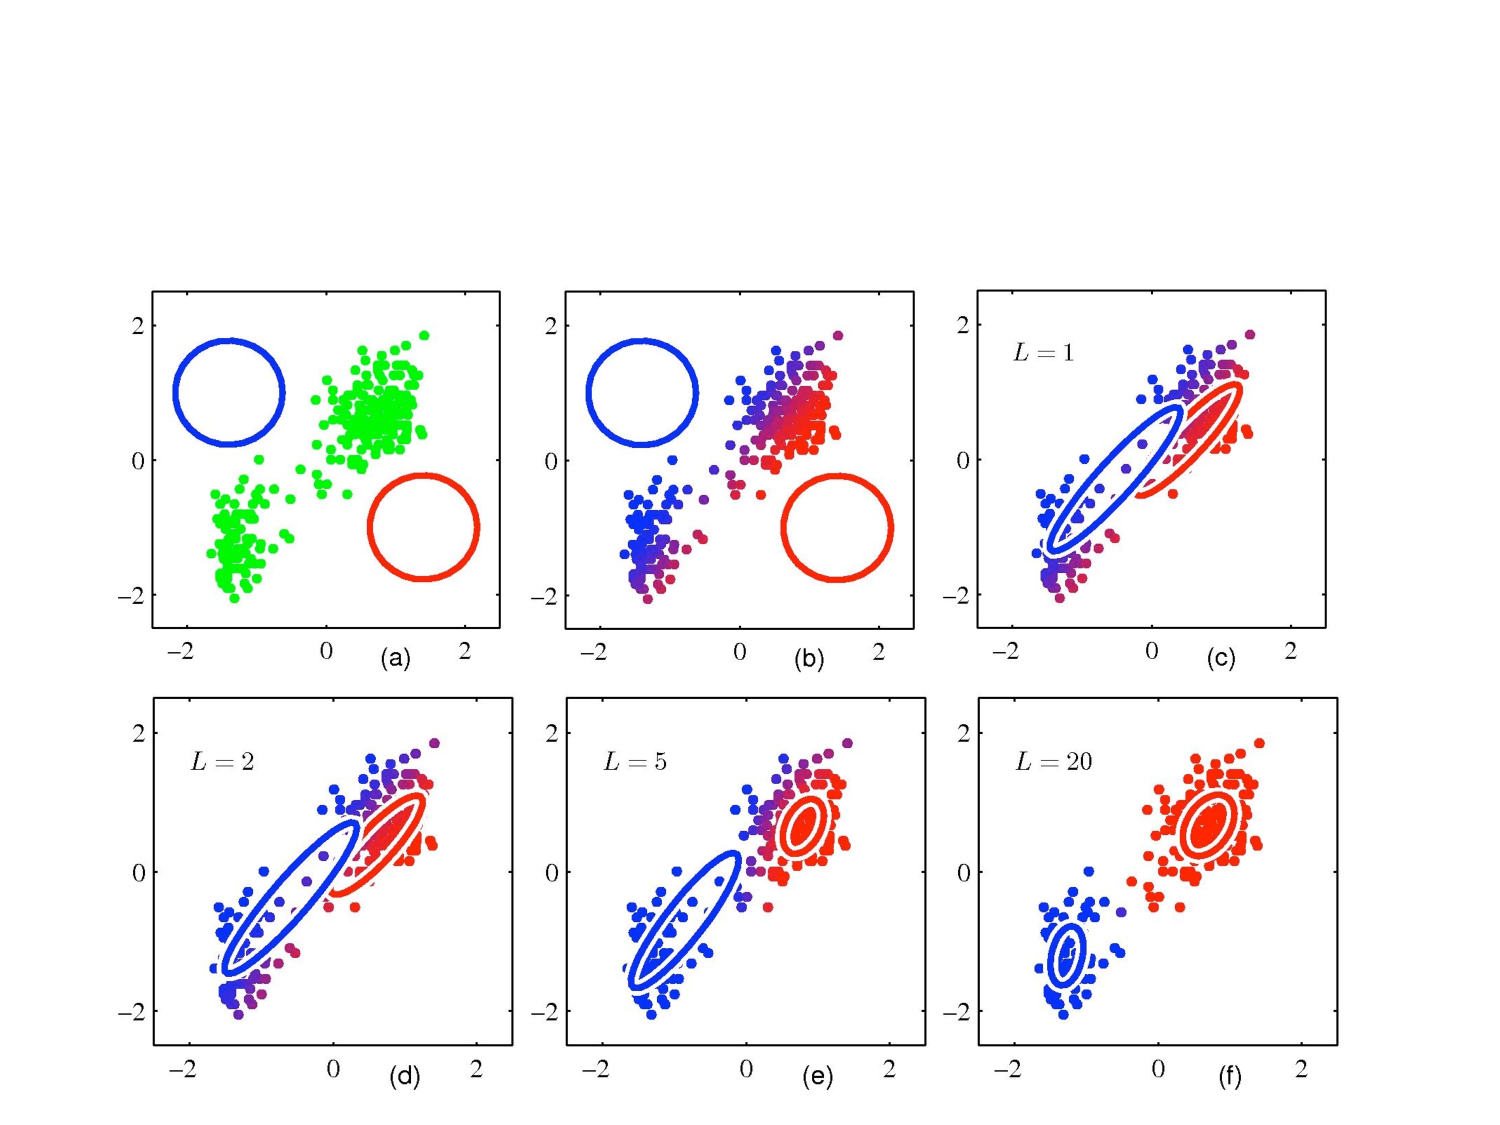
\includegraphics[width=4.2in]{pics/raw3.pdf}
\end{figure}
\end{frame}


\begin{frame}{The General EM algorithm}
Consider a general setting with latent variables.
\begin{itemize}
	\item Observed dataset $\boldsymbol{X}\in \mathbb R^{N\times D}$, latent variables $\boldsymbol{Z}\in \mathbb R^{N\times K}$.
	\end{itemize}
Maximize the log-likelihood  \textcolor{purple}{$\log p(\boldsymbol{X}|\theta)=\log\left(\sum_{\boldsymbol Z}p(\boldsymbol X,\boldsymbol Z|\theta)\right)$}.
\begin{itemize}
	\item Initialize parameters $\theta^{\rm old}$.
%	\item Our knowledge on $z$ carried by the posterior $p(z|x,\theta)$. 
	 \item \textbf{E-step}: use $\theta^{\rm old}$ to compute the posterior $p(\boldsymbol{Z}|\boldsymbol{X},\theta^{\rm old})$.
 	\item \textbf{M-step}: $\theta^{\rm new}=\arg\max_\theta Q(\theta,\theta^{\rm old})$, where
$$
	Q(\theta,\theta^{\rm old})\;=\;\sum_{\boldsymbol{Z}}p(\boldsymbol{Z}|\boldsymbol{X},\theta^{\rm old})\log p(\boldsymbol{X},\boldsymbol{Z}|\theta)\;=\;\mathbb E\Big(\log p(\boldsymbol{X},\boldsymbol{Z}|\theta)\Big|\boldsymbol{X},\theta^{\rm old}\Big)
$$
which is tractable in many applications.
\item Replace $\theta^{\rm old}\leftarrow\theta^{\rm new}$. Repeat until convergence.
\end{itemize}
%\begin{figure}
%\includegraphics[page=19,width=4.8in,trim={0 0 0 3cm},clip]{./raw.pdf}
%\end{figure}
\end{frame}

\begin{frame}{Example: Gaussian mixture}
\begin{itemize}
%	\item We confirm earlier formulas for the Gaussian mixture.
	\item If $z$ was observed, the MLE would be trivial
	$${\small \log p(\boldsymbol X,\boldsymbol Z|\theta)=\sum_{n=1}^N \log p(x_n,z_n|\theta)=\sum_{n=1}^N\sum_{k=1}^K \textcolor{blue}{1\!\!1(z_n\!=\!k)}\log\left(\pi_kN(x_n|\mu_k,\Sigma_k)\right).}$$
\end{itemize}
For the E-step: $p(\boldsymbol{Z}|\boldsymbol{X},\theta)=\prod_{n=1}^N p(z_n|\boldsymbol{X},\theta)$ we have
$$
p(z_n=k|\boldsymbol{X},\theta)=p(z_n=k|x_n,\theta)=\frac{\pi_k N_m(x_n|\mu_k,\Sigma_k)}{\sum_{j=1}^K \pi_j N_m(x_n|\mu_j,\Sigma_j)}.
$$
For the M-step: ${\small \mathbb E(1\!\!1(z_n=k)|\boldsymbol{X},\theta^{\rm old})=p(z_n=k|\boldsymbol{X},\theta^{\rm old})}$ and so 
$$
{\small \mathbb E\Big(\log p(\boldsymbol X,\boldsymbol Z|\theta)\Big|\boldsymbol{X},\theta^{\rm old}\Big)\;=\;\sum_{n=1}^N\sum_{k=1}^K \textcolor{blue}{p(z_n=k|\boldsymbol{X},\theta^{\rm old})}\log\left(\pi_kN(x_n|\mu_k,\Sigma_k)\right).}
$$
Maximizing gives the formulas on Slide~\ref{GMEM}.
%\begin{figure}
%\includegraphics[page=24,width=4.8in,trim={0 0 0 3cm},clip]{./raw.pdf}
%\end{figure}
\end{frame}



\end{document}

